%% Problema: deve essere grassetto nella ToC e nel titolo del capitolo, ma non grassetto nell'header.
\chapter{Signal event selection}
\label{cap:event_selection}
This chapter outlines the three major steps in the selection of \demonstratorshort events for the study of long-lived $\Lambda^0$ baryons in LHCb.
Section \ref{sec:prefilter} discusses the preliminary kinematic variable selections used to provide a loose selection of signal for further analysis;
Section \ref{sec:4:phys_bkg} gives an overview of the two vetoes used to account for the main source of physical background, the \physbkgshort decay;
Section \ref{sec:HBDT} details my work towards the training, optimization and evaluation of a supervised learning multivariate classifier to perform signal-background discrimination;
finally, Section \ref{sec:4:performance_data} brings together all three selection techniques to give proof of \demonstratorshort reconstructibility, fitting the filtered $J/\psi\,\Lambda^0$ invariant mass distributions from simulated signal and Run 2 data.

\section{Prefiltering}
\label{sec:prefilter}
\textit{Prefilters}, also refered to as \textit{preliminary selections} or simply \textit{pre-selections}, are the foundation of the signal selection process.
The main objective of this step is to improve the signal-to-background ratio and reduce the computational workload to analyze data with cuts on kinematic variables.

\begin{table}[t]
	\begin{center}
	\begin{tabular}{@{}llll@{}}
		\toprule
		Variable & Unit & Minimum & Maximum \\
		\midrule
		$p(p)$ 						& MeV/$c$ 	& 2\,000	& 500\,000 \\
		$p_T(p)$ 					& MeV/$c$ 	& 400		& -- \\
		$p(\pi^-)$ 					& MeV/$c$ 	& 10\,000	& 500\,000 \\
		$z_\Lambda^\text{vtx}$		& mm		& 5\,500	& 8\,500 \\
		$p_T(\Lambda^0)$ 			& MeV/$c$ 	& 450		& -- \\
		$m(p\pi^-)$	(Vertex Fitter)	& MeV/$c^2$	& 600		& 1\,500 \\
		$m(p\pi^-)$	(combined)		& MeV/$c^2$	& --		& 2\,000 \\
		$m(p\pi^-)$	(measured)		& MeV/$c^2$	& --		& 1\,500 \\
		$\cos\xi_p (\Lambda^0)$		& --		& 0.9999	& -- \\
		$\Delta \chi^2_\text{PV} (\Lambda^0)$
									& -- 		& --		& 200 \\
		$\chi^2_\text{dist} (\Lambda^0)$
									& --		& --		& $2\times{10}^{7}$ \\
		$\chi^2_\text{vtx} (\Lambda^0)$
									& --		& --		& 750 \\
		$\lvert m(\mu^+ \mu^-) - m_\text{PDG} (J/\psi) \rvert$
									& MeV/$c^2$ & --		& 90 \\
		$m(J/\psi\,\Lambda^0)$ (combined)
									& MeV/$c^2$	& 4\,700		& -- \\
		$m(J/\psi\,\Lambda^0)$ (Vertex Fitter)
									& MeV/$c^2$	& --		& 8\,500 \\
		$\lvert \cos\xi_p (\Lambda^0_b) \rvert$
									& --		& 0.99		& -- \\
		$\Delta \chi^2_\text{PV} (\Lambda^0_b)$
									& -- 		& --		& 1\,750 \\
		$\chi^2_\text{vtx} (\Lambda^0_b)$
									& --		& --		& 150 \\
		\bottomrule
	\end{tabular}
	\end{center}
	\caption{Prefilter selection criteria applied to simulated \demonstratorshort signal and Run 2 data. The Vertex Fitter invariant mass is computed by the homonymous algorithm; the \textit{combined} invariant mass is computed from the 4-momenta of the daughter particles at the first measurement position, without track extrapolation; the \textit{measured} invariant mass is computed in the same way as the combined mass, but after extrapolation at the reconstructed decay vertex of the mother particle. Angle $\xi_p$ for a particle is computed between the line connecting its origin and decay vertices and the direction of its momentum. $\Delta \chi^2_\text{PV}$ is the increase of the primary vertex $\chi^2$ when the particle is included in the fit. $\chi^2_\text{dist}$ is the geometrical distance between the primary vertex and the particle decay vertex in $\chi^2$ units.}
	\label{tab:4:prefilters}
\end{table}

\begin{figure}[t]
	\centering
	\begin{subfigure}{.45\textwidth}
		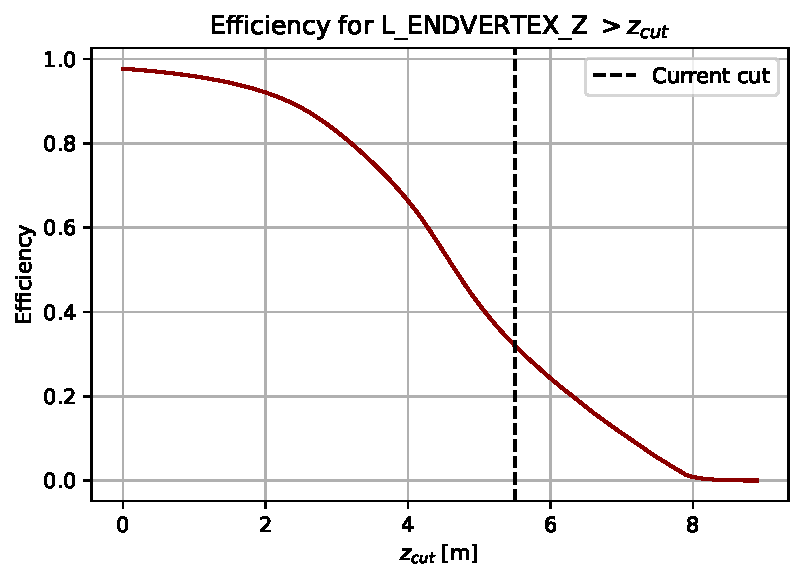
\includegraphics[width=\textwidth]{graphics/04-event_selection/LEVz_left.pdf}
		\caption{}
	\end{subfigure}
	\begin{subfigure}{.45\textwidth}
		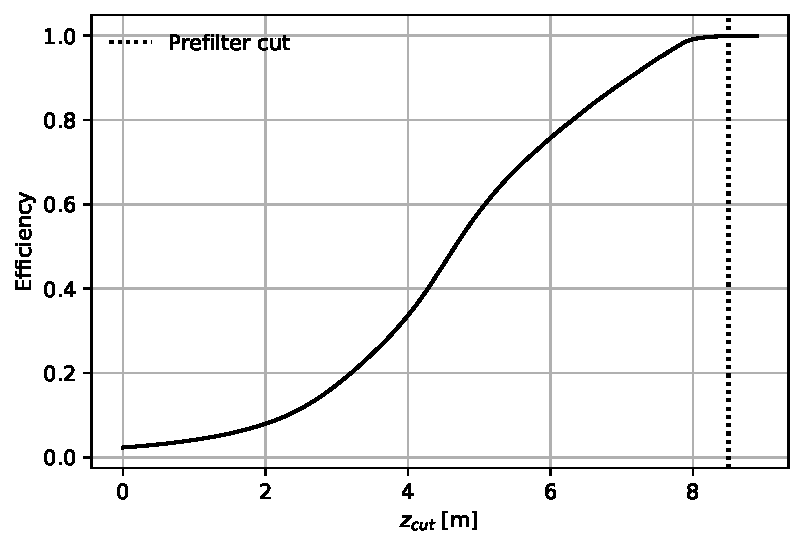
\includegraphics[width=\textwidth]{graphics/04-event_selection/LEVz_right.pdf}
		\caption{}
	\end{subfigure}
	\caption{Efficiency of the $z_\text{vtx}^\Lambda \geq z_\text{cut}^\text{left}$ \textit{(a)} and $z_\text{vtx}^\Lambda \leq z_\text{cut}^\text{right}$ \textit{(b)} prefilter selection criteria on \demonstratorshort simulated signal, as function of the respective thresholds. The \textit{dotted vertical lines} mark the chosen thresholds.}
	\label{fig:4:z_lambda_cuts}
\end{figure}

The applied prefilter criteria are listed in Table \ref{tab:4:prefilters}.
Efficiencies on signal have been estimated with studies on simulated \demonstratorshort events.
The most impactful selection is the one applied to $z_\text{vtx}^\Lambda$, the $z$ component of the \lambdadecay decay vertex;
the efficiencies for the left and right cuts as a function of the threshold are shown in Figure \ref{fig:4:z_lambda_cuts}.
Since I require $\Lambda^0$ to decay after the dipole magnet in order to observe spin precession, the $\approx 32\%$ efficiency of the $z_\text{vtx}^\Lambda \geq \SI{5.5}{\meter}$ cut cannot be avoided.
Other selections have a much lower impact on signal, with efficiencies $\gtrsim 80\%$, resulting in a total prefilter efficiency of $\approx 26\%$.

As detailed in Section \ref{sec:2:tracking}, a key aspect of my analysis is the employment of T tracks for the reconstruction of the \lz.
The low residual magnetic field for protons and pions produced far from the dipole magnet lowers momentum resolution for the associated tracks down to $20$--$30\%$.
Resolution can be improved up to $\approx 10\%$ by placing kinematic constraints on $p\pi^-$ and $\mu^+ \mu^-$ invariant masses, fixing them to the PDG values of $m(\Lambda^0)$ and $m(J/\psi)$ respectively (these will be henceforth referred to as \textit{mass constraints}).
This approach cannot be implemented in the leaf-by-leaf framework of the default Vertex Fitter algorithm for vertex reconstruction;
instead each event is refitted with the Decay Tree Fitter (DTF) algorithm in two configurations, single $J/\psi$ and double $J/\psi\,\Lambda^0$ mass constraints (see also Section \ref{sec:3:dtf}).

A convergence requirement of the DTF algorithm with the $J/\psi\,\Lambda^0$ mass constraints is therefore added to the prefilter selections.
The main drawback of this selection, a steep 45\% efficiency on simulated signal events (although raised to 65\% when only considering events passing the non-DTF prefilters), is outweighed by the benefits of the improved momentum resolution in the determination of the angular distribution of \lambdadecay decay products.

\section{Physical background rejection}
\label{sec:4:phys_bkg}
%Most physics analyses conducted with hadron colliders are up against two different sources of background with the same (or similar) final state as the searched signal:
%\begin{enumerate}
%	\item \textit{combinatorial} background denotes events where the particles are produced 
%	\item \textit{physical} background denotes events where 
%\end{enumerate}

The main source of physical background for the \demonstratorfull decay is the similar
\begin{equation}
	B^0 \rightarrow J/\psi~(\rightarrow \mu^+ \mu^-)~K_S^0~(\rightarrow \pi^+ \pi^-).
\end{equation}
The final states of the two decays only differ for a $p \leftrightarrow \pi^+$ change.
The \kshort meson also has comparable mean lifetime to the \lz, thus we expect a sizeable number of \kshort decaying after the dipole magnet.
To top it off, the \bz mass (\SI{5279.65}{\mev\per c\squared}) is fairly close to that of \lbz (\SI{5619.60}{\mev\per c\squared}) \cite{PDG}, muddying the waters in invariant mass fits.

As discussed in Section \ref{sec:2:pid}, the LHCb detector employs the two RICH systems to identify and distinguish between protons, pions and kaons;
in the case of $\Lambda^0$ decaying after the dipole magnet RICH1 contributions is impossible, but information from RICH2 would still be available for the vast majority of the decays at hand.
Unfortunately, this is where the experimental nature of physics analyses with T tracks becomes relevant once again:
due to technical issues in the implementation, RICH2 information for particle identification is unavailable for T tracks recorded during LHC Runs 1 and 2\footnote{A large effort by the Milan and Valencia LHCb research groups is underway at the time of writing to implement RICH2 information in T track trigger lines for Run 3.}, making \physbkgshort discrimination much more difficult.

\subsection{Invariant mass veto with pion mass hypothesis}
\label{sec:B0_veto}

\begin{figure}[t]
	\centering
	\begin{subfigure}{.45\textwidth}
		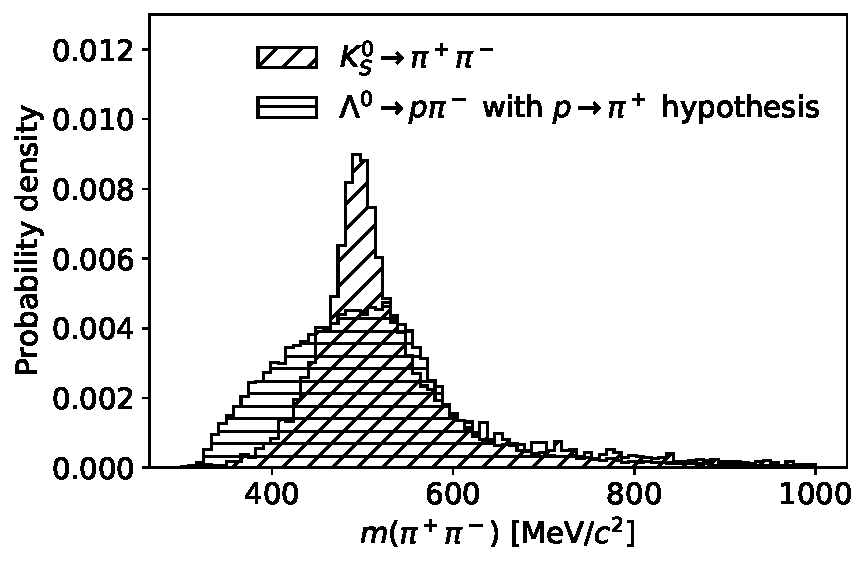
\includegraphics[width=\textwidth]{graphics/04-event_selection/phys_bkg_ks_comparison.pdf}
		\caption{}
		\label{fig:4:phys_bkg_ks}
	\end{subfigure}
	\begin{subfigure}{.45\textwidth}
		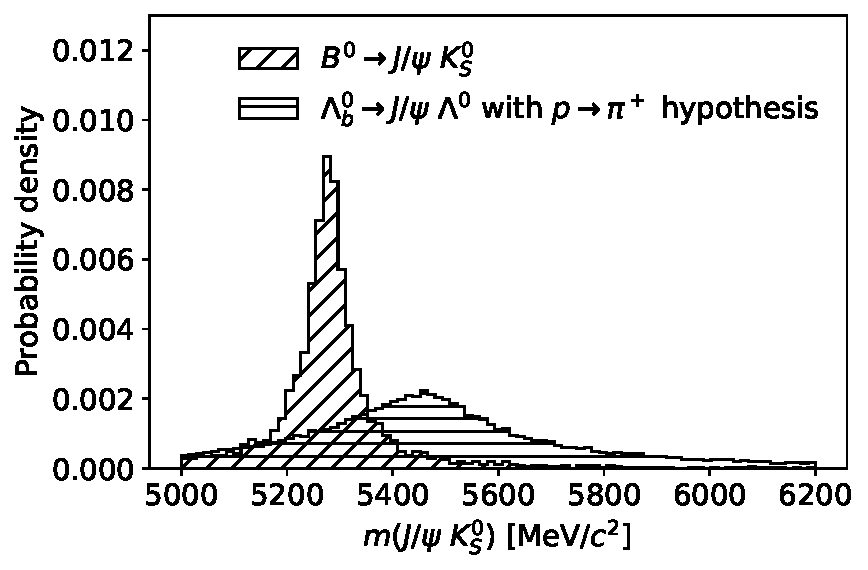
\includegraphics[width=\textwidth]{graphics/04-event_selection/phys_bkg_b0_comparison.pdf}
		\caption{}
		\label{fig:4:phys_bkg_b0}
	\end{subfigure}
	\caption{Comparison of simulated $m(\pi^+\pi^-)$ \textit{(a)} and $m(J/\psi~K^0_S)$ \textit{(b)} distributions: \demonstratorshort events with $p\rightarrow \pi^+$ mass hypothesis are labeled by \textit{horizontal hatching}, \physbkgshort events by \textit{diagonal hatching}.}
	\label{fig:4:phys_bkg_distributions}
\end{figure}

%To address this issue, events must pass a physical background selection based on the results of a Decay Tree Fitter refit with $p\rightarrow \pi^+$ mass hypothesis and kinematic constraints on the $J/\psi$ and $K_S^0$ invariant masses.

For the first step in \bz background rejection, all events are refit with the Decay Tree Fitter algorithm using \jpsi and \kshort invariant mass constraints and a $p \rightarrow \pi^+$ mass hypothesis, i.e. assuming that the proton is a misclassified pion and fitting the entire decay tree as such.
The veto rejects an event if the DTF refit converges and $m(J/\psi~K_S^0)$ is too close in value to the $B^0$ PDG mass, that is
\begin{equation}
	\lvert
	m(J/\psi~K_S^0) - m_\text{PDG}(B^0)
	\rvert < m_\text{thres},
\end{equation}
with tunable threshold $m_\text{thres}$.

This approach was tested on simulated \demonstratorshort and \physbkgshort samples.
The variable $m(J/\psi~K_S^0)$ was chosen as opposed to $m(\pi^+\pi^-)$ due to the significant overlap between $m(\pi^+\pi^-)$ invariant mass distributions of actual $K_S^0 \rightarrow \pi^+ \pi^-$ events and \lambdadecay events with $p\rightarrow \pi^+$ mass hypothesis (Figure \ref{fig:4:phys_bkg_ks});
the $m(J/\psi~K_S^0)$ distributions are comparatively more separate (Figure \ref{fig:4:phys_bkg_b0}), allowing for a better selection on the variable.

\begin{figure}[t]
	\centering
	\begin{subfigure}{.45\textwidth}
		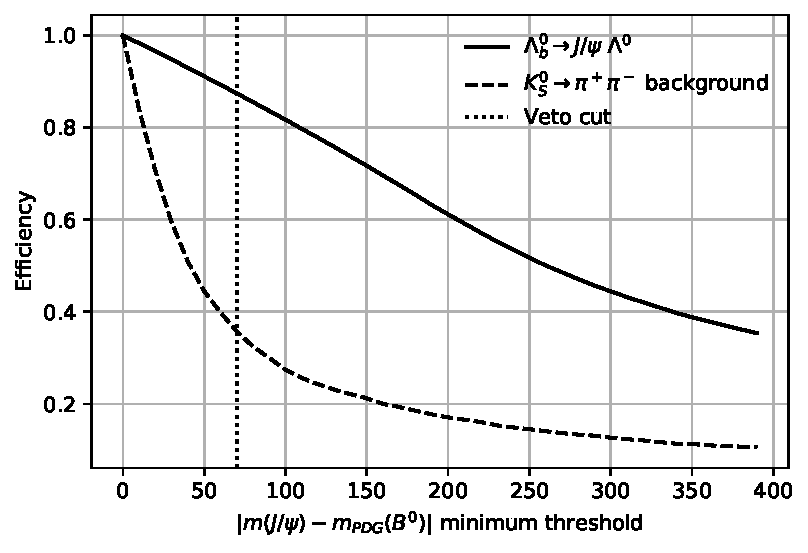
\includegraphics[height=.2\textheight]{graphics/04-event_selection/phys_veto_efficiencies.pdf}
		\caption{}
		\label{fig:4:phys_bkg_veto_eff_thres}
	\end{subfigure}
	\begin{subfigure}{.45\textwidth}
		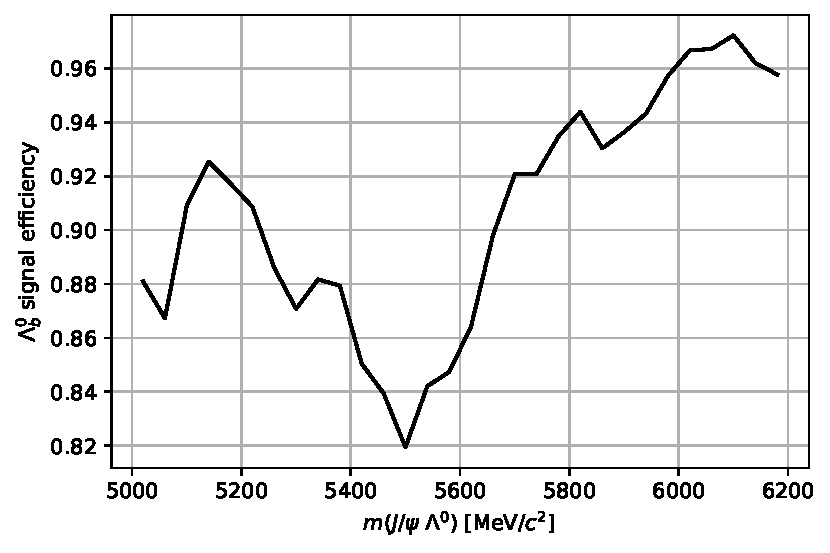
\includegraphics[height=.2\textheight]{graphics/04-event_selection/phys_veto_sig_efficiencies_per_bin.pdf}
		\caption{}
		\label{fig:4:phys_bkg_veto_eff_mass}
	\end{subfigure}
	\caption{\textit{(a)} Efficiency of physical background veto as a function of the invariant mass discrepancy threshold on simulated signal (\demonstratorshort, \textit{solid}) and background (\physbkgshort with proton mass hypothesis, \textit{dashed}) events. Chosen threshold marked by \textit{dotted line}. \textit{(b)} Efficiency of the veto on different $m(J/\psi\,\Lambda^0)$ bins for \demonstratorshort signal events.}
	\label{fig:4:phys_bkg_veto_eff}
\end{figure}

Figure \ref{fig:4:phys_bkg_veto_eff_thres} shows the veto efficiency on \demonstratorshort signal and \physbkgshort physical background as function of the threshold $m_\text{thres}$.
The chosen value of $m_\text{thres} = \SI{70}{\mev}$ retains 87\% of signal while rejecting 64\% of background;
signal efficiency as function of the $m(J/\psi\,\Lambda^0)$ invariant mass is depicted in Figure \ref{fig:4:phys_bkg_veto_eff_mass}.

\subsection{Armenteros-Podolanski veto}
To supplement the invariant mass veto, I introduced a selection criterium on proton and pion momenta based on the Armenteros-Podolanski technique \cite{armenteros-podolanski}.
This approach, first proposed in 1954, allows for momentum-based discrimination of \lambdadecay and \kshortdecay decays without the need for mass assumptions on the daughter particles.

\begin{figure}[t]
	\centering
	\begin{subfigure}{.45\textwidth}
		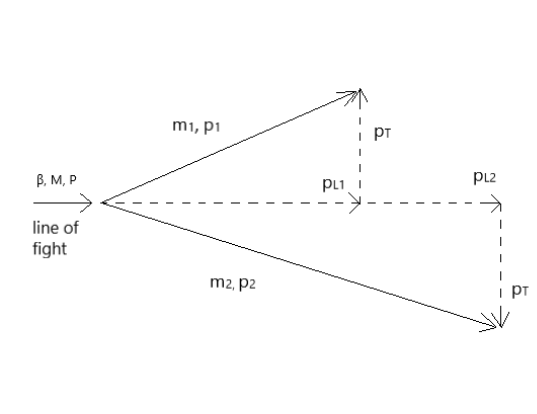
\includegraphics[height=.24\textheight]{graphics/04-event_selection/twobody_labframe.png}
		\caption{}
		\label{fig:4:twobody_labframe}
	\end{subfigure}
	\begin{subfigure}{.45\textwidth}
		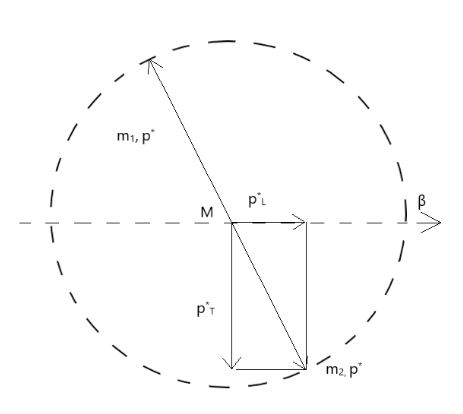
\includegraphics[height=.24\textheight]{graphics/04-event_selection/twobody_cmframe.png}
		\caption{}
		\label{fig:4:twobody_cmframe}
	\end{subfigure}
	\caption{Two-body decay kinematics in the laboratory \textit{(a)} and center-of-mass \textit{(b)} reference frames \cite{armenteros_calibration}.}
	\label{fig:4:twobody_frames_ap}
\end{figure}

%\begin{equation}
%{p^\star} ^2 =
%\frac{1}{4M^2}
%\left(
%	M^4 +m_1^4 + m_2^2 - 2m_1^2 M^2 - 2m_2^2 M^2 - 2m_1^2 m_2^2
%\right)
%\end{equation}

Let $M \rightarrow m_1 m_2$ be a two-body decay, shown in the laboratory frame in Figure \ref{fig:4:twobody_labframe};
given the mother particle line of flight, we define longitudinal momentum \pl and transverse momentum \pt for the two daughter particles, with $p_\text{T}^{(1)} = - p_\text{T}^{(2)} \equiv p_\text{T}$.
These quantities can be expressed in terms of their values in the center-of-mass frame of the decay (Figure \ref{fig:4:twobody_cmframe}) with a Lorentz $\beta$ boost along the $M$ momentum:
\begin{subequations}
\label{eq:4:ap_p_lorentz}
\begin{align}
	p_\text{L} &= \gamma \left( p_\text{L}^\star + \beta E^\star \right)
	\label{eq:4:ap_pL_lorentz} \\
	p_\text{T} &= p_\text{T}^\star.
	\label{eq:4:ap_pT_lorentz}
\end{align}
\end{subequations}
Energy $E^\star$ of the daughter particles in the center-of-mass frame are known for two-body decays to be
\begin{subequations}
\label{eq:4:ap_Estar}
\begin{align}
	E_1^\star &=
	\frac{1}{2M}
	\left(M^2 + m_1^2 - m_2^2 \right), \\
	%%%%%%%%%%%%%%%%%%%%%%%%%%%%%%%%%%%%%
	E_2^\star &=
	\frac{1}{2M}
	\left(M^2 - m_1^2 + m_2^2 \right)
\end{align}
\end{subequations}
In turn, \plstar and \ptstar are related to the momentum modulus $p^\star \coloneqq \lvert \vec{p}^\star \rvert$ of the daughter particle, which is fixed by two-body decay kinematics, via the angle $\theta$ between $\vec{p}^\star_{(1)}$ and $\vec{\beta}$:
\begin{subequations}
\label{eq:4:ap_p_theta}
\begin{align}
	p_\text{L}^\star &= \pm p^\star \cos\theta,	\label{eq:4:ap_pL_theta} \\
	p_\text{T}^\star &= p^\star \sin\theta.		\label{eq:4:ap_pT_theta}
\end{align}
\end{subequations}

The Armenteros-Podolanski technique exploits the predictable physics of a two-body decay in the Armenteros-Podolanski space defined by the longitudinal momentum asymmetry
\begin{equation}
	\alpha \coloneqq
	\frac
	{p_\text{L}^{(1)} - p_\text{L}^{(2)}}
	{p_\text{L}^{(1)} + p_\text{L}^{(2)}},
	\label{eq:4:ap_alpha}
\end{equation}
and transverse momentum \pt of the decay.
Substituting \eqref{eq:4:ap_pL_lorentz}, \eqref{eq:4:ap_p_theta} and \eqref{eq:4:ap_Estar} into \eqref{eq:4:ap_alpha} we obtain
\begin{equation}
\alpha =
\frac{m_1^2 - m_2^2}{M^2}
+
\frac{2p^\star}{\beta M} \cos\theta
\equiv
\alpha_0 + \frac{r_\alpha}{\beta} \cos\theta,
\label{eq:4:ap_alpha_theta}
\end{equation}
with
\begin{equation}
\alpha_0 \coloneqq \frac{m_1^2 - m_2^2}{M^2}
\end{equation}
and
\begin{equation}
r_\alpha \coloneqq \frac{2p_\star}{M}.
\end{equation}
Result \eqref{eq:4:ap_alpha_theta} can further be combined with \eqref{eq:4:ap_pT_theta} through the Pythagorean trigonometric identity
\begin{equation}
\cos^2 \theta + \sin^2 \theta = 1,
\end{equation}
yielding
\begin{equation}
\frac
{\left( \alpha - \alpha_0 \right)^2}
{r_\alpha^2}
+
\frac{p_\text{T}^2}{{p^\star}^2}
= 1.
\label{eq:4:ap_ellipse}
\end{equation}

\begin{figure}[t]
	\centering
	\begin{subfigure}{.45\textwidth}
		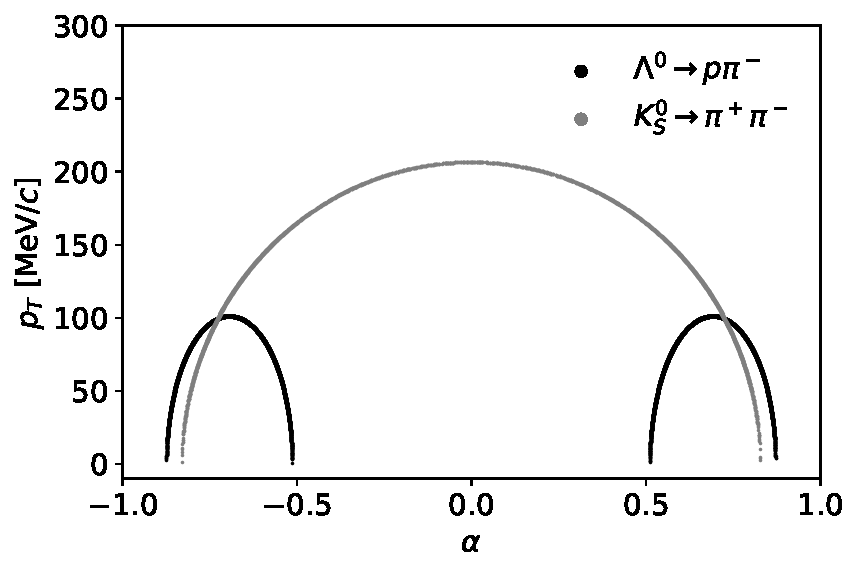
\includegraphics[height=.2\textheight]{graphics/04-event_selection/MCTRUTH_armenteros_podolanski_MC_scatter.pdf}
		\caption{}
		\label{fig:4:ap_plots_truth}
	\end{subfigure}
	\begin{subfigure}{.45\textwidth}
		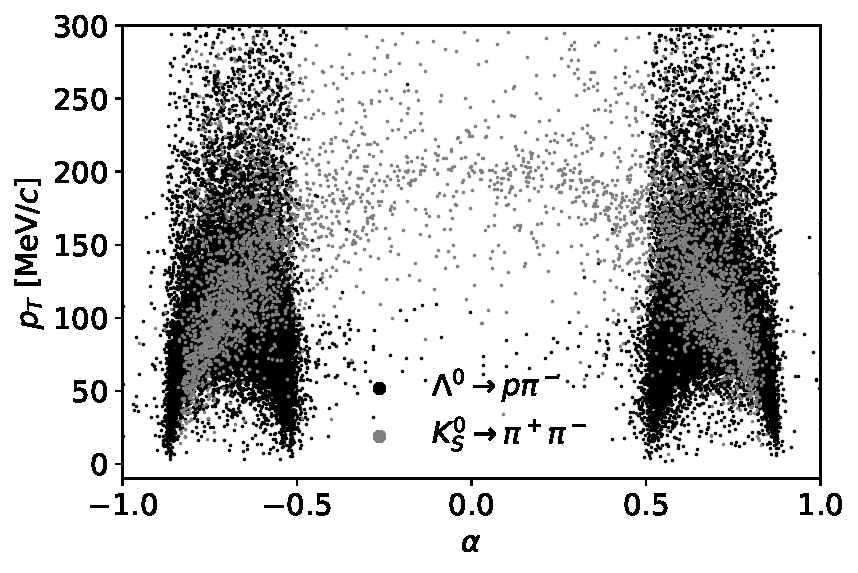
\includegraphics[height=.2\textheight]{graphics/04-event_selection/DTF_FixJPsi_armenteros_podolanski_MC_scatter.pdf}
		\caption{}
		\label{fig:4:ap_plots_dtf}
	\end{subfigure}
	\caption{Armenteros-Podolanski plots for simulated \demonstratorshort (\textit{black}) and \physbkgshort (\textit{grey}) events, using true momenta \textit{(a)} and Decay Tree Fitter momenta with \jpsi mass constraint \textit{(b)}. Longitudinal \pl and transverse \pt momenta are defined here with respect to the \lz/\kshort lines of flight, with \pl asymmetry $\alpha$ defined as in equation \eqref{eq:4:ap_alpha}.}
	\label{fig:4:ap_plots_mc}
\end{figure}

We have thus shown that momenta of daughter particles from a two-body decay define an ellipse in the $\alpha$--\pt Armenteros-Podolanski space, with center and radii depending on particle masses and momentum distributions.
This is verified in Figure \ref{fig:4:ap_plots_truth}, which shows the $\alpha$--\pt scatterplot of \lambdadecay (\kshortdecay) decays from simulated \demonstratorshort (\physbkgshort) events, computed with true momenta.
In this case $\alpha$ is conventionally computed assigning the positive particle to $m_1$, which corresponds to $p$ in \lz decays and $\pi^+$ in $\bar{\Lambda}^0$ and \kshort decays, leading to the two symmetrical ellipses for the \demonstratorshort events.

While a selection criterium based on the \kshort and \lz ellipses would appear trivial, momentum resolution needs to be taken into account.
Figure \ref{fig:4:ap_plots_dtf} shows the Armenteros-Podolanski space for the same events using momenta reconstructed with the Decay Tree Fitter algorithm with \jpsi mass constraint\footnote{While the additional \lz mass constraint used so far drastically improves momentum resolution in \demonstratorshort events, applying it to \physbkgshort events is detrimental as it distorts the Armenteros-Podolanski phase space, making \kshortdecay events overlap with the \lambdadecay ellipses.}.
The significant overlap of the two classes of events prevents selection criteria on the \pt axis, but still allows for a criterium on $\alpha$ relatively devoid of false positives.

\begin{figure}[t]
	\centering
	\begin{subfigure}{.45\textwidth}
		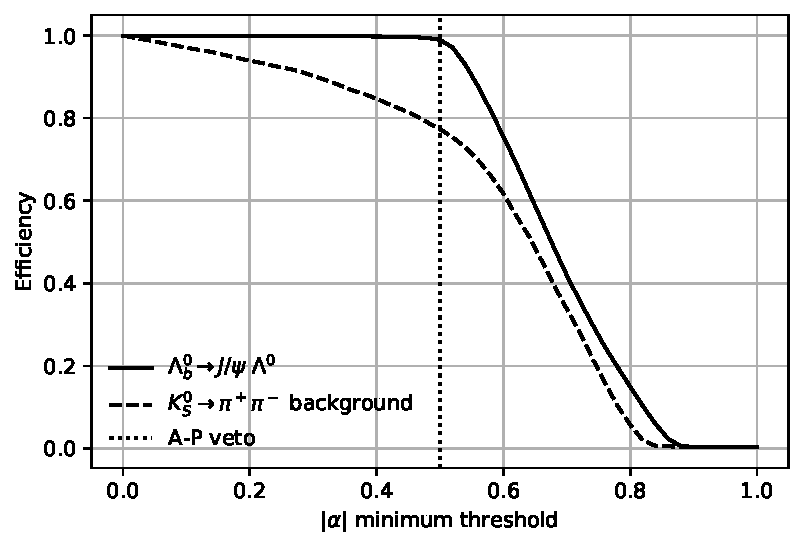
\includegraphics[height=.2\textheight]{graphics/04-event_selection/ap_efficiencies.pdf}
		\caption{}
		\label{fig:4:ap_efficiency}
	\end{subfigure}
	\begin{subfigure}{.45\textwidth}
		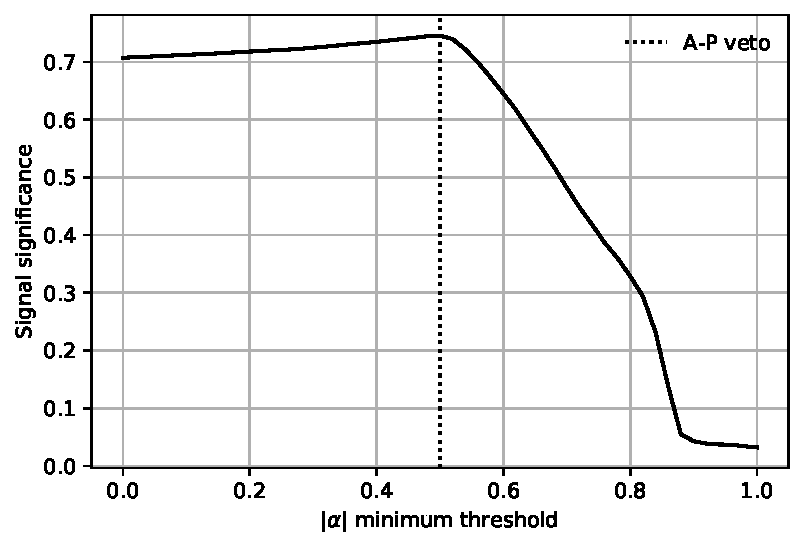
\includegraphics[height=.2\textheight]{graphics/04-event_selection/ap_significances.pdf}
		\caption{}
		\label{fig:4:ap_significance}
	\end{subfigure}
	\caption{\textit{(a)} Efficiency of Armenteros-Podolanski veto as a function of the $|\alpha|$ threshold on simulated signal (\demonstratorshort, \textit{solid}) and background (\physbkgshort, \textit{dashed}) events. \textit{(b)} Signal significance as a function of the $|\alpha|$ threshold. The chosen threshold in both plots is marked by the \textit{dotted line}.}
	\label{fig:4:ap_threshold_optimization}
\end{figure}

Given the symmetrical nature of the Armenteros-Podolanski space, I implemented the veto in the form
\begin{equation}
|\alpha| \geq \alpha_\text{thres}.
\end{equation}
I optimized the $\alpha_\text{thres}$ threshold to maximize \demonstratorshort signal significance
\begin{equation}
\frac{s}{\sqrt{s+b}}.
\label{eq:4:signal_significance}
\end{equation}
Usually $s$ and $b$ would be the signal and background event counts after the selection;
since yields in Run 2 data are still unknown at this selection step, I instead used the fraction of total signal and physical background events after loose and invariant mass veto selections also passing the Armenteros-Podolanski veto with a specific threshold.

Figure \ref{fig:4:ap_efficiency} shows the signal and background efficiencies of the veto as a function of $\alpha_\text{thres}$, while Figure \ref{fig:4:ap_significance} reports the corresponding signal significances.
The chosen threshold of 0.5 retains 99\% of the \demonstratorshort signal while rejecting 23\% of \physbkgshort background surviving the \bz veto described in Section \ref{sec:B0_veto}.
In addition, the Armenteros-Podolanski veto will also remove combinatorial \kshortdecay events which the \bz veto, being based on the $J/\psi\,K_S^0$ invariant mass, is not equipped to deal with.

\section{HBDT classifier}
\label{sec:HBDT}
Even after prefilter selections, combinatorial background exceeds the signal by a ${10}^3$ factor.
This section details my work in training and testing a multivariate classifier to discriminate \demonstratorshort events, in order to lower the signal-to-background ratio to acceptable levels for physics analysis.
After taking into consideration a wide range of classifiers, a histogram-based gradient boosting classification tree (also referred to as \textit{histogram-based boosted decision tree}, HBDT for short) was chosen by virtue of its superior performance in studies on sample data \cite{Pessina:BSc:2020}.
Training, optimization and performance testing of the classifier were made with the Scikit-learn 0.24.2 package \cite{scikit-learn} for Python 3.6.8 \cite{10.5555/1593511}.

\begin{figure}
	\centering
	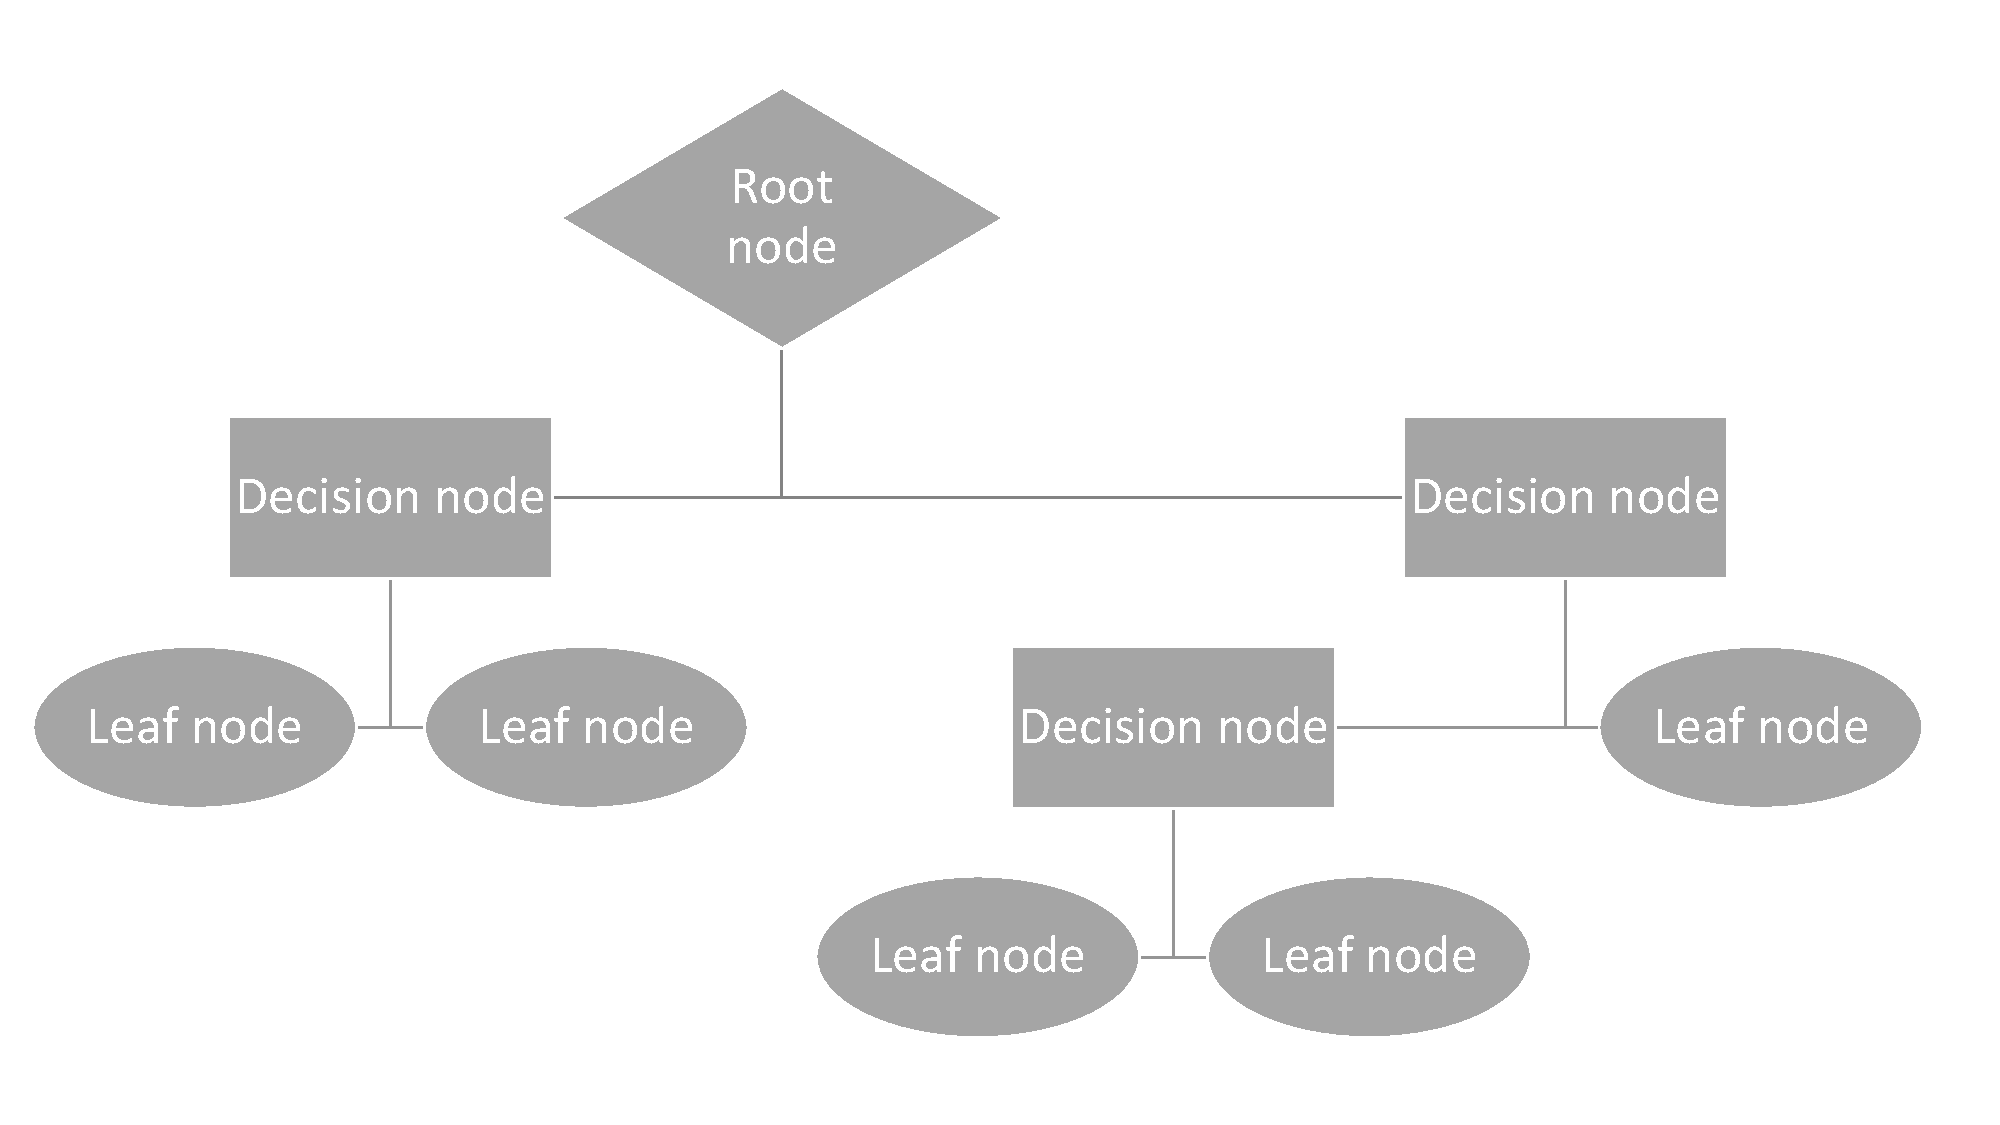
\includegraphics[height=.3\textheight]{graphics/04-event_selection/decision_tree.pdf}
	\caption{Diagrammatic representation of a decision tree classifier.}
	\label{fig:4:decision_tree}
\end{figure}

The basic layout of a binary decision tree classifier is sketched in Figure \ref{fig:4:decision_tree}:
a sequence of decision nodes applies binary conditions according to available information on the individual event and eventually reaches a leaf node associated to the \textit{event score} $t$, in this case the probability that the event is a \demonstratorshort decay.
Performance of the decision tree can be enhanced with \textit{boosting} \cite{Yann:2013}, whereby the ultimate classifier is built as a weighted average of a large number of weaker trees;
the result is known as a boosted decision tree (BDT).
In the adaptive boosting (AdaBoost) implementation used in this thesis, each tree $T_k$ is trained on a reweighted data sample that prioritizes events misclassified by tree $T_{k-1}$.
The usage of a histogram-based BDT, arranging input samples into integer-valued bins, allows for much faster estimators when working with large data samples ($n \gtrsim {10}^4$).

%(gradient tree boosting with logistic loss function for binary classification)

\subsection{Training and testing data}
\label{sec:4:train_test_data}

\begin{figure}[t]
	\centering
	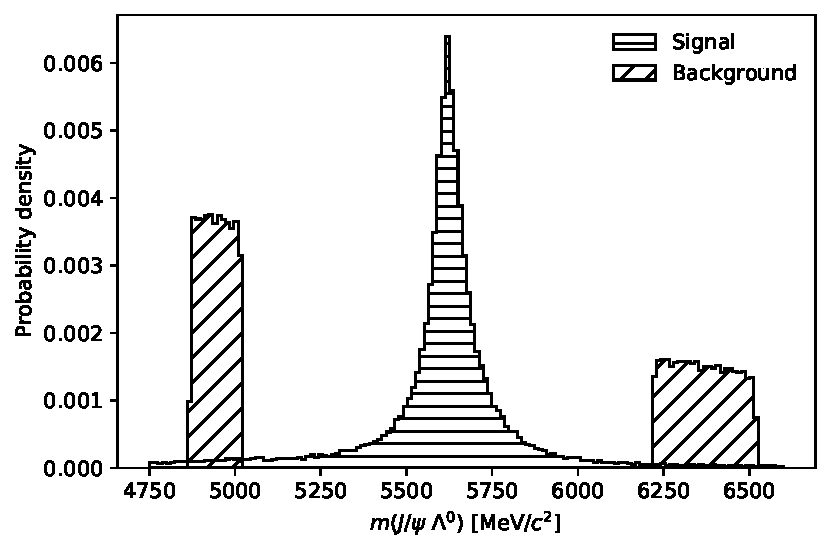
\includegraphics[width=.6\textwidth]{graphics/04-event_selection/sig_bkg_distribution_balance.pdf}
	\caption{Signal (\textit{horizontal hatching}) and background (\textit{diagonal hatching}) data samples used for training the HBDT classifier.
	%Test samples are taken from the same pool in 1:9 ratio.
	}
	\label{fig:4:HBDT_training_data}
\end{figure}

Supervised training of a classifier requires signal and background datasets as input to learn to distinguish between the two classes.
For signal I used simulated \demonstratorshort events, while for the background I sampled side bands on the left ($\left[\SI{4870.2}{\mev \per c^2}, \SI{5020.2}{\mev \per c^2}\right]$) and right ($\left[\SI{6220.2}{\mev \per c^2}, \SI{6520.2}{\mev \per c^2}\right]$) of the expected \lbz peak  in the Run 2 data $m(J/\psi\,\Lambda)$ distribution (see Figure \ref{fig:4:HBDT_training_data}).

I considered two options for the signal-to-background ratio:
\begin{itemize}
	\item \textit{balanced} training dataset: $\approx 145\,000$ events, evenly split between signal and background;
	\item \textit{unbalanced} training dataset: $\approx 73\,000$ signal events, $\approx 3.6$ million background events.
\end{itemize}
The standard approach to machine learning calls for a roughly balanced dataset to train the classifier on signal and background alike.
Given the disproportionate signal-to-background ratio in the case at hand, however, I also explored the unbalanced approach, aiming for improved background rejection at the price of (reasonably) subpar signal identification.
Classifiers trained with balanced or unbalanced datasets showed very similar performances after score threshold optimization (see Section \ref{sec:4:threshold_optimization}), the main difference being that balanced HBDTs require harsher score selection criteria;
since no reason surfaced to favour either approach, I opted to follow the more conventional path and empolyed a balanced training dataset.
Testing data for performance evaluation was sampled from the same pool as training data in a 1:9 ratio.

The following kinematic variables (also known as \textit{features}) were used for signal discrimination:
transverse and longitudinal momenta of $p$, \pim and \jpsi;
coordinates of the \lambdadecay vertex position;
\lbz and \lz pointing angles $\xi_p$, i.e. the angle between the particle line of flight and its momentum;
$\tilde{\chi}^2_\text{vtx}$ of the \demonstratorshort and \lambdadecay vertices;
the increase $\Delta \chi^2_\text{PV}$ of the primary vertex $\chi^2$ when a particle is included in the fit, for \lbz and \lz;
the distances $\chi^2_\text{dist}$ between \lbz and \lz decay vertices and the primary vertex in $\chi^2$ units.

The momenta for proton and pion are computed with $J/\psi$ mass constraints.
While the usage of $p,\pi^-$ momenta from the Decay Tree Fitter with the additional $\Lambda^0$ mass constraint was considered, preliminary tests on classifiers showed a slight degradation of their performance when the double mass constraint was adopted.
The standard Vertex Fitter momenta were used for the $J/\psi$ on account of the already great resolution provided by using Long muons.

\subsection{Hyperparameter optimization}
\label{sec:4:hyperoptimization}

The supervised training process for a classifiers tunes a set of parameters to minimize a given loss function; in the HBDT case, decision node and tree weights are trained according to the output of a logistic loss function.
In contrast, \textit{hyperparameters} are parameters governing the learning process itself and thus require separate optimization.

I selected three hyperparameters for optimization:
\begin{itemize}
	\item learning rate $L \in [0.003, 0.006, 0.010, 0.015]$, the shrinkage factor for the contribution of each tree in the boosting process.
	\item maximum number of boosting iterations $n_\text{max}^\text{iter} \in [1500, 2500, 5000]$;
	\item maximum number of leaves for each tree $n_\text{max}^\text{leaves} \in [100, 200, 400, 800]$.
\end{itemize}
Other hyperparameters, such as the maximum number of bins and the minimum number of samples per leaf, were left as the default values of the Scikit-learn implementation.

I performed an exhaustive grid scan of the aforementioned hyperparameter values.
Each classifier was evaluated on training data using a stratified $k$-folds cross validation technique: the training sample is split in $k=5$ subsamples, the classifier is trained in rotation on $k-1$ samples and tested with the $k$-th, and the $k$ results are averaged together.
For a given score threshold $i$, we define \textit{precision} $P_i$ and \textit{recall} $R_i$ in terms of the true/false positive/negative rates: precision 
\begin{equation}
	P_i = \frac{n_\text{TP}}{n_\text{TP} + n_\text{FP}}
	\label{eq:4:precision}
\end{equation}
scores how often the classifier mistakes background for signal, while recall
\begin{equation}
	R_i = \frac{n_\text{TP}}{n_\text{TP} + n_\text{FN}}
	\label{eq:4:recall}
\end{equation}
scores how well the classifier is able to recognize the signal.
Performance of cross-validated classifiers on training and testing sub-samples\footnote{Still working within a cross-validation mindset, here \textit{testing data} is used to refer to the $k$-th fold in the cross-validation. No actual testing data as defined in Section \ref{sec:4:train_test_data} was used for the hyperoptimization step.} was evaluated using the \textit{average precision} figure of merit
\begin{equation}
	\text{AP} = \sum_{i=2}^{n} (R_i - R_{i-1})P_i
	\label{eq:4:average_prec}
\end{equation}
for a set of $n$ thresholds.

When considering the choice of the best classifier, I aimed to strike a balance between the AP score on testing data, acting as a raw performance grading of the classifier, and the difference in AP score between training and testing samples, which was necessary to prevent overtraining.
The HBDT classifier used for the remainder of this thesis, with $L=0.003$, $n_\text{max}^\text{iter}=2500$, and $n_\text{max}^\text{leaves}=100$, is the result of this selection process.

\subsection{Performance test}

\begin{figure}[t]
	\centering
	\begin{subfigure}{.45\textwidth}
		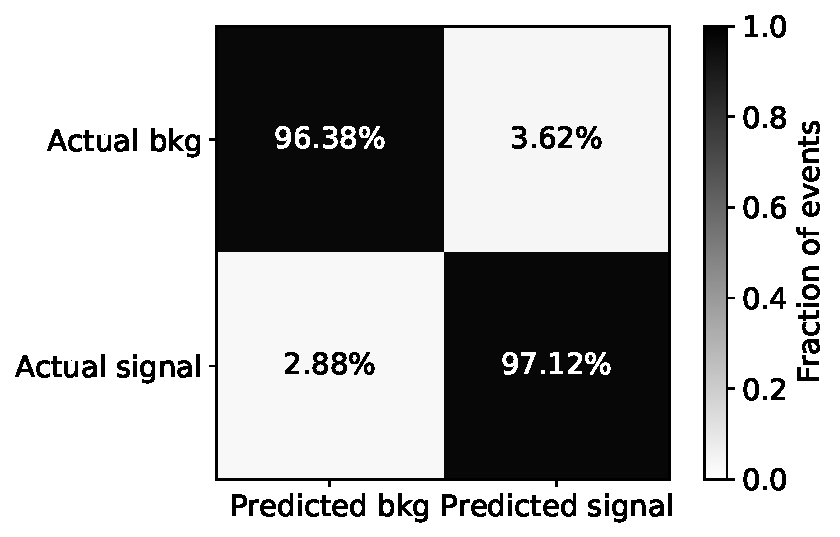
\includegraphics[width=\textwidth]{graphics/04-event_selection/confmatrix_train.pdf}
		\caption{}
	\end{subfigure}
	\begin{subfigure}{.45\textwidth}
		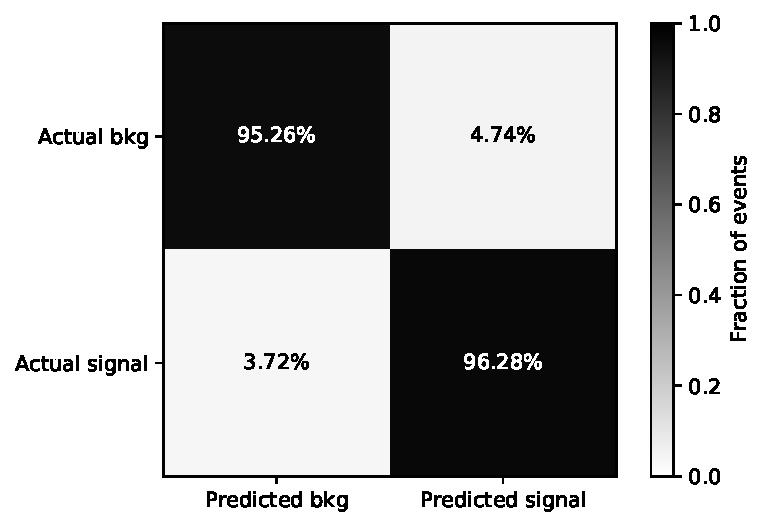
\includegraphics[width=\textwidth]{graphics/04-event_selection/confmatrix_test.pdf}
		\caption{}
	\end{subfigure}
	\caption{Confusion matrices visualizing the performance of the HBDT classifier on training \textit{(a)} and testing \textit{(b)} data samples. Percentages and chromatic scale are normalized to the true event classification: for instance, the top left and top right quadrants of a matrix represent the fraction of true background events reconstructed as background or signal, respectively. Binary classification uses an illustrative response threshold $t_\text{thres} = 0.5$.}
	\label{fig:4:confusion_matrix}
\end{figure}

Performance of the trained HBDT optimized as per Section \ref{sec:4:hyperoptimization} was evaluated on the smaller test sample described in Section \ref{sec:4:train_test_data}.
Figure \ref{fig:4:confusion_matrix} shows the confusion matrices for training and test data with a score threshold of $t_\text{thres}=0.5$, meaning events with $t>t_\text{thres}$ are classified as signal.
The matrices summarize the true/false positive/negative rates for the classifier, highlighting the expected slight dip in accuracy when moving from training to test sample.

\begin{figure}[t]
	\centering
	\begin{subfigure}{.45\textwidth}
		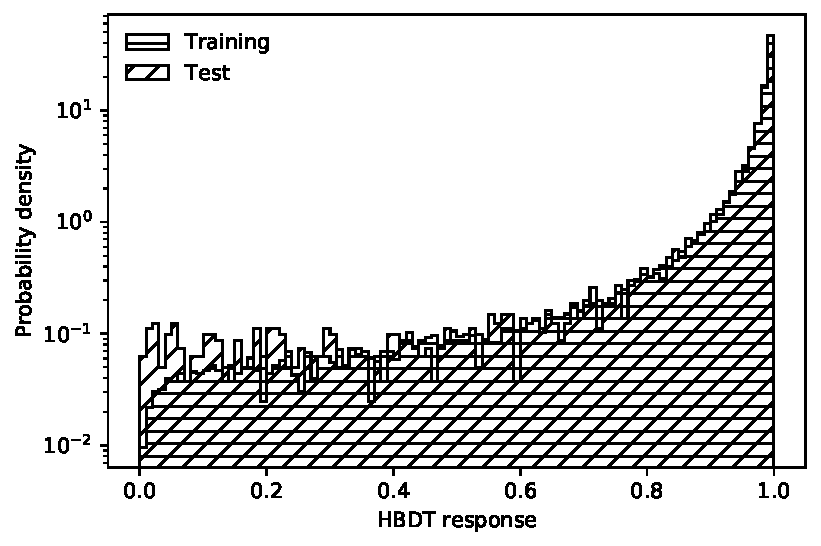
\includegraphics[width=\textwidth]{graphics/04-event_selection/sig_train_vs_test.pdf}
		\caption{}
		\label{fig:4:sig_train_vs_test}
	\end{subfigure}
	\begin{subfigure}{.45\textwidth}
		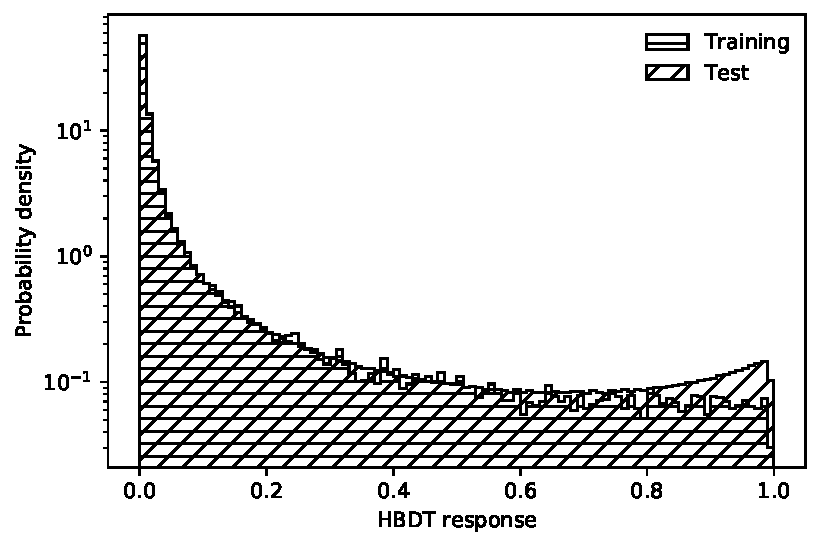
\includegraphics[width=\textwidth]{graphics/04-event_selection/bkg_train_vs_test.pdf}
		\caption{}
		\label{fig:4:bkg_train_vs_test}
	\end{subfigure}
	\caption{Response distribution of the HBDT classifier on signal \textit{(a)} and background \textit{(b)} events. The training sample is represented by \textit{horizontal hatching}, the test sample by \textit{diagonal hatching}.}
	\label{fig:4:train_vs_test}
\end{figure}

Comparing the signal and background score distributions (Figures \ref{fig:4:sig_train_vs_test} and \ref{fig:4:bkg_train_vs_test} respectively) for training and test data samples, I observed a light discrepancy at the end tails.
Such a split in favour of performance on training data is usually an early indicator of ovetraining.
I investigated this possibility by conducting a two-sample Kolmogorov-Smirnov (K-S) test \cite{10.2307/2280095}, which computes the probability $p$ that two samples are drawn from the same probability distribution.
Conventionally, the K-S is considered passed if $p>0.05$;
this was true for both signal ($p_\text{sig} \approx 0.30$) and background ($p_\text{bkg} \approx 0.07$), confirming that the classifier is not significantly ovetrained.

\begin{figure}
	\centering
		\begin{subfigure}{.45\textwidth}
		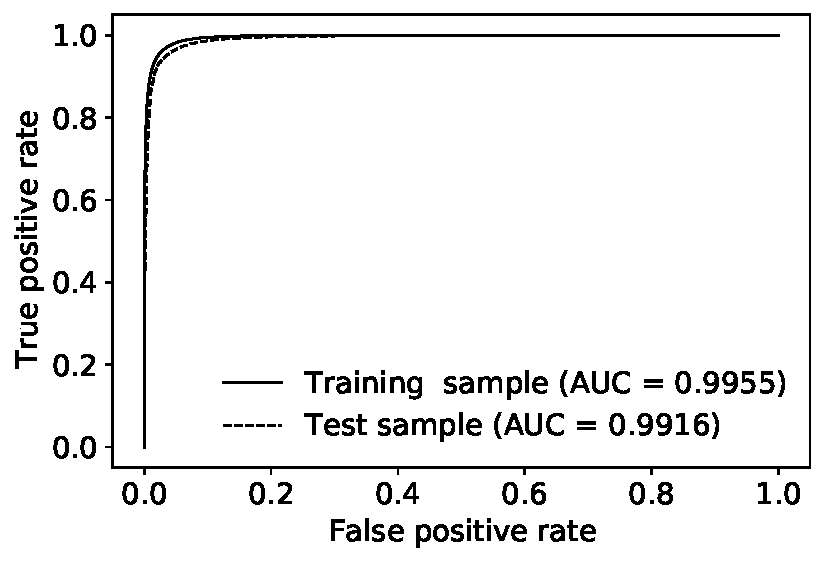
\includegraphics[width=\textwidth]{graphics/04-event_selection/roc.pdf}
		\caption{}
		\label{fig:4:hbdt_roc_curve}
	\end{subfigure}
	\begin{subfigure}{.45\textwidth}
		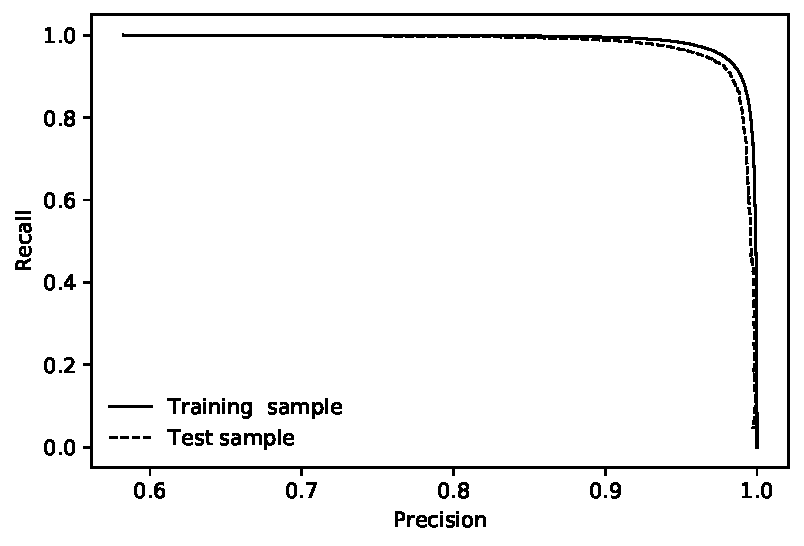
\includegraphics[width=\textwidth]{graphics/04-event_selection/prec_recall.pdf}
		\caption{}
		\label{fig:4:hbdt_precall_curve}
	\end{subfigure}
	\caption{Receiving operating characteristic (ROC) curve \textit{(a)} and precision-recall curve \textit{(b)} for the HBDT classifier on training (\textit{solid}) and test (\textit{dashed}) samples. The legend in the ROC plot includes the area-under-curve (AUC) score.}
	\label{fig:4:hbdt_performance_curves}
\end{figure}

I assessed the classifier performance at different thresholds using the receiving operating characteristic (ROC) and precision-recall curves.
The ROC curve, depicted in Figure \ref{fig:4:hbdt_roc_curve}, plots the true positive versus false positive rates for a set of thresholds left as hidden variables:
a random classifier would bisect the plot plane, while a perfect classifier would adhere to the axes and cross the $(0,1)$ point.
The integral below the curve is itself a figure of merit, the area-under-curve (AUC), with better classifiers scoring values closer to unity.
The precision-recall curve follows a similar principle to the ROC curve, plotting precision \eqref{eq:4:precision} and recall \eqref{eq:4:recall} for different thresholds;
in this case, a perfect classifier would cross the $(1,1)$ point.
In both instances, the classifier shows great performance and high consistency between training and test samples.

\begin{figure}
	\centering
	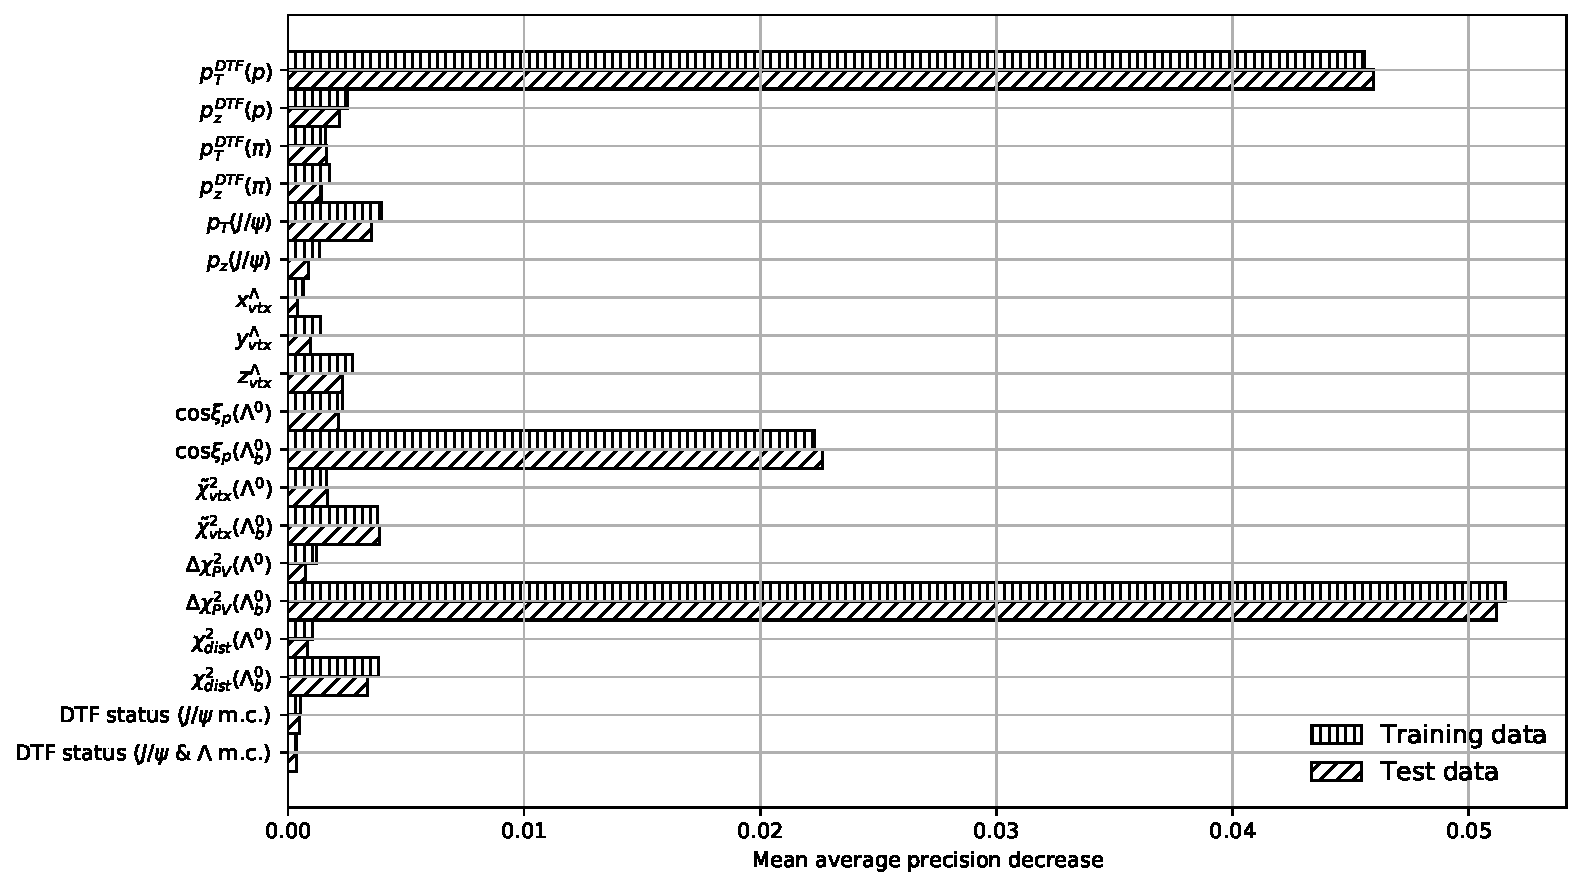
\includegraphics[width=\textwidth]{graphics/04-event_selection/importances.pdf}
	\caption{Decrease in the HBDT AP score when permutating the values of individual features in training (\textit{vertical hatching}) and testing (\textit{diagonal hatching}) data samples. See the legend of Table \ref{tab:4:prefilters} for details on the feature labels.}
	\label{fig:4:hbdt_importances}
\end{figure}

Finally, I evaluated the importance of selected features in signal discrimination.
This was achieved by permutating the values of each feature at a time and evaluating the average decrease in the baseline AP score of the classifier over ten of such permutations.
Results are shown in Figure \ref{fig:4:hbdt_importances} for training and testing samples:
in both cases the most discriminating features, causing the largest drops in AP, are the transverse momentum of the proton, the pointing angle of the $\Lambda_b^0$ and the increase in the primary vertex $\chi^2$ when including the $\Lambda_b^0$ in the fit.

\subsection{Threshold optimization}
\label{sec:4:threshold_optimization}

The final step in the classifier tuning process was the optimization of the threshold to maximize signal significance \eqref{eq:4:signal_significance} after the HBDT filter.
A simple way to do it would be to fit the $J/\psi\,\Lambda^0$ invariant mass distribution of filtered data with signal and background functions and extract the corresponding rates via integration;
however, this has the undesired side effect of heightening the risk of biasing the selection towards our specific data sample.
%A different, more general approach was devised instead.

A different, more general approach was devised to prevent this.
I first identified a <<soft>> score threshold $t_\text{thres} = 0.7$, just high enough for the filtered Run 2 data $m(J/\psi\,\Lambda^0)$ distribution (using values from Decay Tree Fitter with mass constraints on both \lbz daughters) to show the \lbz resonance peak.
I fit the simulated signal $m(J/\psi\,\Lambda^0)$ distribution with a double-tailed asymmetric Crystal Ball function.
The standard, single-tailed Crystal Ball probability density function is parameterized as
\begin{equation}
	f_\text{CB}(m; \mu, \sigma, \alpha, n) =
	\begin{cases}
		\exp\left[ -\frac{1}{2} {\left(\frac{m-\mu}{\sigma}\right)}^2 \right],
		& \text{if } \frac{m-\mu}{\sigma} \geq -\alpha \\
		A \cdot {\left(B - \frac{m-\mu}{\sigma}\right)}^{-n},
		& \text{if } \frac{m-\mu}{\sigma} < -\alpha
	\end{cases},
	\label{eq:4:crystal_ball}
\end{equation}
with
\begin{equation}
	A = {\left(\frac{n}{|\alpha|}\right)}^n~e^{-\frac{\alpha^2}{2}}
\end{equation}
and
\begin{equation}
	B = \frac{n}{|\alpha|} - |\alpha|.
\end{equation}
Its shape is thus a Gaussian core with a power-law tail on the lower end when $m$ outdistances $\mu$ by $\alpha\sigma$.
The double-tailed Crystal Ball expands on this concepts by having a Gaussian core with two asymmetric long tails, governed by different power laws:
\begin{equation}
	f_\text{sig}
	\left(m; S, \mu, \sigma, \alpha_1, n_1, \alpha_2, n_2 \right) =
	N
	\begin{cases}
	f_\text{CB}(m; \mu, \sigma, \alpha_1, n_1)
	& \text{if } m \leq \mu \\
	f_\text{CB}(2\mu -m; \mu, \sigma, \alpha_2, n_2)
	& \text{if } m > \mu \\
	\end{cases},
\end{equation}
with normalization
\begin{equation}
	N = \frac{S}{\sigma(C_1 + C_2 + D)}
\end{equation}
itself depending on
\begin{equation}
	C_1 = \frac{n_1}{\alpha_1 (n_1-1)} e^{-\frac{\alpha^2_1}{2}},
\end{equation}
\begin{equation}
	C_2 = \frac{n_2}{\alpha_2 (n_2-1)} e^{-\frac{\alpha^2_2}{2}},
\end{equation}
and
\begin{equation}
	D = \sqrt{2\pi} \left(G_\text{c} (\alpha_2) - G_\text{c} (- \alpha_1)\right),
\end{equation}
where
\begin{equation}
G_\text{c}(x) \coloneqq \frac{1}{\sqrt{2\pi}} \int_{-\infty}^x dt\,e^{-\frac{t^2}{2}}
\end{equation}
is the Gaussian cumulative distribution function evaluated at $x$.

When fitting $m(J/\psi\,\Lambda^0)$ in Run 2 data, the function is the sum of two contributions:
signal is modeled with the same double-tailed Crystal Ball from \eqref{eq:4:crystal_ball}, with all parameters bar $S$ and $\sigma$ fixed to their Monte Carlo fit best values;
the combinatorial background is fit with a conventional exponential function
\begin{equation}
	f_\text{bkg} (m;C,a) = C e^{-a m}.
	\label{eq:4:exponential}
\end{equation}
As will be shown in Section \ref{sec:4:performance_data}, the outlined combination of $f_\text{sig}$ and $f_\text{bkg}$ provides an excellent description of Run 2 data, as long as sufficient filtering is applied for the $\Lambda_b^0$ peak to emerge.

This data fit provides preliminary $s_0$ and $b_0$ values, obtained by integrating signal and background fit functions in the $\pm 3\sigma$ region around $\mu$.
I used these values to estimate the signal (background) rate $s_i$ ($b_i$) for events passing a score threshold $t_i$ with associated efficiency $\varepsilon_i^s$ ($\varepsilon_i^b$):
\begin{subequations}
\begin{align}
	s_i &= s_0 \frac{\varepsilon_i^s}{\varepsilon_0^s}, \\
	b_i &= b_0 \frac{\varepsilon_i^b}{\varepsilon_0^b}.
\end{align}
\end{subequations}
Here $\varepsilon_0^s$ and $\varepsilon_0^b$ are the signal and background efficiencies associated to the soft threshold with $s_0$ and $b_0$ rates.
Efficiencies were computed on the test sample and correspond to true/false positive rates evaluated for the ROC curve (Figure \ref{fig:4:hbdt_roc_curve}).

\begin{figure}
	\centering
	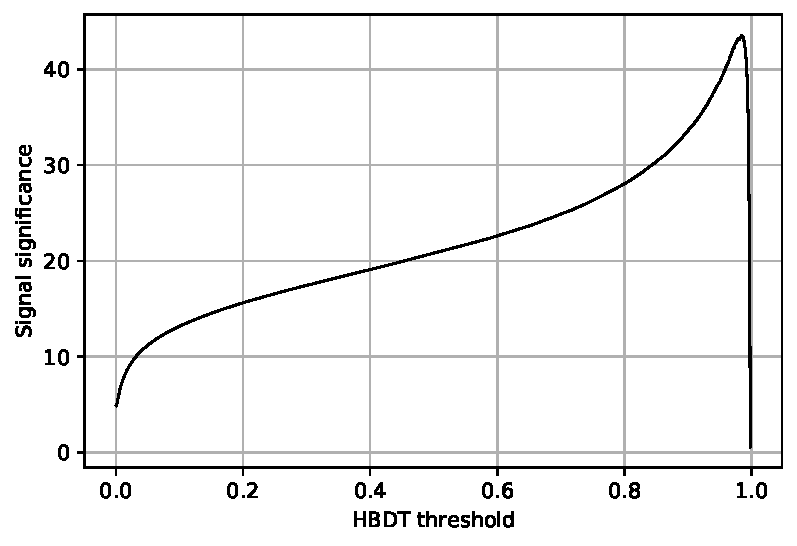
\includegraphics[width=.6\textwidth]{graphics/04-event_selection/HBDT_signal_significance.pdf}
	\caption{Projected \demonstratorshort signal significance over background as a function of the HBDT response threshold used for selection.}
	\label{fig:4:signal_significance}
\end{figure}

Using the estimated $s_i$ and $b_i$, I calculated the predicted signal significance \eqref{eq:4:signal_significance} for each threshold $t_i$.
Figure \ref{fig:4:signal_significance} shows the results as a function of the score threshold.
The best performing threshold was found to be $t_\text{thres} = 0.985$, with signal significance $\approx 46$ and signal purity
\begin{equation}
	\frac{s}{s+b} \approx 0.6.
\end{equation}

\section{Signal yield in invariant mass fits}
\label{sec:4:performance_data}

\begin{figure}[t]
	\centering
	\begin{subfigure}{.45\textwidth}
		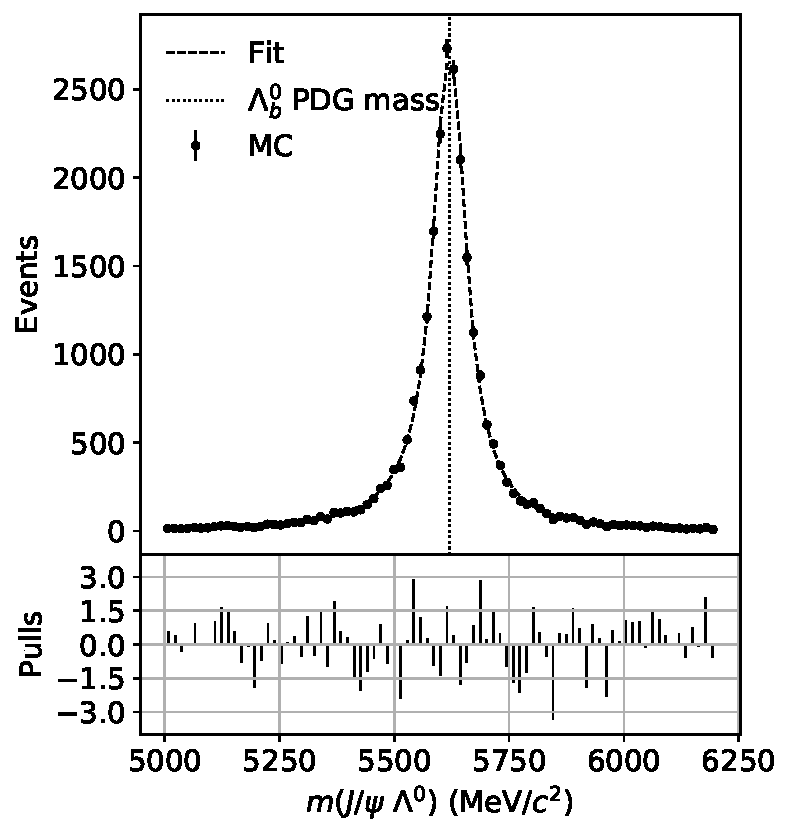
\includegraphics[width=\textwidth]{graphics/04-event_selection/MC_lambdab_hard_fit.pdf}
		\caption{}
		\label{fig:4:mc_fit}
	\end{subfigure}
	\begin{subfigure}{.45\textwidth}
		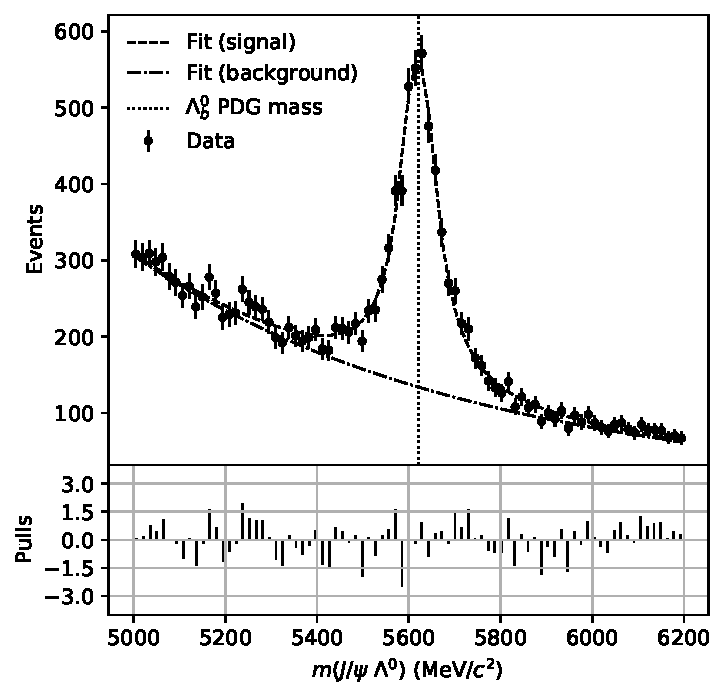
\includegraphics[width=\textwidth]{graphics/04-event_selection/data_lambdab_hard_fit.pdf}
		\caption{}
		\label{fig:4:data_fit}
	\end{subfigure}
	\caption{Fitted $m(J/\psi\,\Lambda^0)$ invariant mass distributions for simulated \demonstratorshort events \textit{(a)} and Run 2 data \textit{(b)} after all selection steps. Signal fit function is \textit{dashed}, background fit function in \textit{(b)} is \textit{dash-dotted}. The PDG value for the $\Lambda_b^0$ mass \cite{PDG} is marked by the \textit{dotted vertical line}. Fit pulls (data-fit discrepancy divided by uncertainty) are shown below the main plots.}
\end{figure}

\begin{table}
	\begin{center}
	\begin{tabular}{@{}llllllll@{}}
		\toprule
		Parameter
		& Unit
		& \multicolumn{2}{c}{Simulation}	& \phantom{a}
		& \multicolumn{2}{c}{Data} \\
		\cmidrule{3-4} \cmidrule{6-7}
		&& Best value	& Error				&& Best value	& Error \\
		\midrule
		$S$			& --		& 365\,900	& 3\,100&& 65\,600	& 1\,800	\\
		$\mu$		& MeV/$c^2$	& 5\,620.2 	& 0.6	&& 5\,620.2	& -- 		\\
		$\sigma$	& MeV/$c^2$	& 36.9		& 1.0	&& 41.6		& 1.6		\\
		$\alpha_1$	& --		& 0.99		& 0.04	&& 0.99	& --		\\
		$n_1$		& --		& 2.44		& 0.12	&& 2.44		& --		\\
		$\alpha_2$	& --		& 1.01		& 0.04	&& 1.01	& --		\\
		$n_2$		& --		& 2.69		& 0.15	&& 2.69		& --		\\
		$C$			& --		& --		& --	&& 240,000	& 40\,000	\\
		$a$			& $\times {10}^{-3}~\text{MeV}^{-1}c^2$
								& --		& --	&& 1.336	& 0.029		\\
		\bottomrule
	\end{tabular}
	\end{center}
	\caption{Parameter best values and associated uncertainties from $m(J/\psi\,\Lambda^0)$ fits on simulated signal and Run 2 data, after all selection steps. Parameters with no reported error are fixed.}
	\label{tab:4:fit_results}
\end{table}

Figures \ref{fig:4:mc_fit} and \ref{fig:4:data_fit} show the $m(J/\psi\,\Lambda^0)$ invariant mass distributions of Monte Carlo simulated signal and Run 2 data after applying prefilters, \physbkgshort vetoes and the optimized $t > 0.985$ selection on the HBDT classifier score.
To fit the distributions I adopted the same approach outlined in Section \ref{sec:4:threshold_optimization}:
the simulated signal is described with the double-tailed asymmetric Crystal Ball \eqref{eq:4:crystal_ball};
the best fit parameter values, except for $S$ and $\sigma$, are fixed for the signal function in the Run 2 data fit, while the exponential \eqref{eq:4:exponential} was used to model the combinatorial background.

Binned fit results are listed in Table \ref{tab:4:fit_results}.
The employed functions provide a great description for both the Monte Carlo simulation and the real data from Run 2, as seen from the fit-data discrepancies consistently below $3\sigma$ for each data bin.
The resolution of the resonance peak is $\approx 12\%$ worse in real data compared to the simulation, an expected consequence of the underlying combinatorial background.
Integrating the functions in the $\mu \pm 3\sigma$ interval, we estimate a $3590 \pm 60$ signal event yield and $2420 \pm 50$ background event yield.
These are going to be the baseline yields for analyses on the $\Lambda^0$ electromagnetic dipole moments.